\documentclass[12pt,a4paper]{article}

% ── Packages ──────────────────────────────────────────────────────────────────
\usepackage[a4paper, margin=2.5cm]{geometry}
\usepackage[T1]{fontenc}
\usepackage[utf8]{inputenc}
\usepackage{lmodern}
\usepackage{amsmath, amssymb}
\usepackage{booktabs}
\usepackage{array}
\usepackage{tabularx}
\usepackage{longtable}
\usepackage{parskip}
\usepackage{hyperref}
\usepackage{xcolor}
\usepackage{titlesec}
\usepackage{enumitem}
\usepackage{listings}
\usepackage{microtype}
\usepackage{fancyhdr}
\usepackage{lastpage}
\usepackage{graphicx}
\usepackage{float}

% ── Hyperref setup ────────────────────────────────────────────────────────────
\hypersetup{
    colorlinks=true,
    linkcolor=blue!70!black,
    urlcolor=blue!70!black,
    citecolor=blue!70!black,
    pdftitle={COS 710 Assignment 1 -- Genetic Programming for Symbolic Regression},
    pdfauthor={Yohali Malaika Kamangu}
}

% ── Header / Footer ───────────────────────────────────────────────────────────
\pagestyle{fancy}
\fancyhf{}
\rhead{COS 710 -- Assignment 1}
\lhead{Yohali Malaika Kamangu (u23618583)}
\cfoot{\thepage\ of \pageref{LastPage}}
\renewcommand{\headrulewidth}{0.4pt}

% ── Section title formatting ──────────────────────────────────────────────────
\titleformat{\section}{\large\bfseries}{}{0em}{\thesection.\quad}
\titleformat{\subsection}{\normalsize\bfseries}{}{0em}{\thesubsection\quad}

% ── Code listing style ────────────────────────────────────────────────────────
\lstset{
    basicstyle=\ttfamily\small,
    breaklines=true,
    frame=single,
    backgroundcolor=\color{gray!8},
    rulecolor=\color{gray!40},
    xleftmargin=1em,
    xrightmargin=1em
}

% ── Column type for tables ────────────────────────────────────────────────────
\newcolumntype{L}[1]{>{\raggedright\arraybackslash}p{#1}}
\newcolumntype{C}[1]{>{\centering\arraybackslash}p{#1}}
\newcolumntype{R}[1]{>{\raggedleft\arraybackslash}p{#1}}

% ══════════════════════════════════════════════════════════════════════════════
\begin{document}

% ── Title Page ────────────────────────────────────────────────────────────────
\begin{titlepage}
    \centering
    \vspace*{2cm}
    {\LARGE\bfseries COS 710: Artificial Intelligence\par}
    \vspace{0.5cm}
    {\Large Assignment 1: Genetic Programming for Symbolic Regression\par}
    \vspace{2cm}
    \begin{tabular}{ll}
        \textbf{Module}         & COS 710 --- Artificial Intelligence \\[4pt]
        \textbf{Assignment}     & Assignment 1 \\[4pt]
        \textbf{Due Date}       & 16 March 2026 \\[4pt]
        \textbf{Student Name}   & Yohali Malaika Kamangu \\[4pt]
        \textbf{Student Number} & u23618583 \\
    \end{tabular}
    \vfill
\end{titlepage}

\tableofcontents
\newpage

% ══════════════════════════════════════════════════════════════════════════════
\section*{Introduction}
\addcontentsline{toc}{section}{Introduction}

Accurate forecasting of residential electricity demand is a problem with direct practical implications: from scheduling power generation to managing grid stability, knowing what load to expect at a given time influences a wide range of operational decisions. Time series prediction methods are therefore widely studied across both classical statistics and computational intelligence.

This assignment applies \textbf{Genetic Programming (GP)} to symbolic regression on a real-world residential energy dataset from the United Kingdom. Rather than fitting parameters to a pre-specified model, symbolic regression searches the space of mathematical expressions itself. GP is well suited to this: it evolves arithmetic expression trees through natural selection analogues --- tournament selection, subtree crossover, and subtree mutation --- without any assumption about the functional form of the relationship between variables.

The objective is to evolve a closed-form expression that predicts the electricity load at time $t$ using the $n$ most recent observed load values. The entire implementation was written from scratch in Java, with no external GP frameworks or machine learning libraries, and was evaluated across 10 independent runs on 100,000 rows of the six-year dataset.

% ── Problem Description ───────────────────────────────────────────────────────
\section*{Problem Description}
\addcontentsline{toc}{section}{Problem Description}

The task is an \textbf{autoregressive time series prediction} problem. The target variable is \texttt{Electricity\_load} at time $t$, and the predictors are the $n$ most recently observed load values immediately before $t$. Using a sliding window of size $n = 7$, each example takes the form:

\begin{center}
\begin{tabular}{ll}
\toprule
\textbf{Input} & \textbf{Meaning} \\
\midrule
$x_1$ & Load$(t-1)$ --- most recent \\
$x_2$ & Load$(t-2)$ \\
$x_3$ & Load$(t-3)$ \\
$x_4$ & Load$(t-4)$ \\
$x_5$ & Load$(t-5)$ \\
$x_6$ & Load$(t-6)$ \\
$x_7$ & Load$(t-7)$ --- oldest in the window \\
Target $y$ & Load$(t)$ \\
\bottomrule
\end{tabular}
\end{center}

The GP system evolves expressions of the form $\hat{y} = f(x_1, \ldots, x_7)$ where $f$ is a binary expression tree discovered through evolution.

% ══════════════════════════════════════════════════════════════════════════════
\section{Dataset Description}

The dataset is the \textbf{Residential Energy Usage UK (2014--2020)} dataset, recording electricity consumption from a residential property in the United Kingdom at \textbf{15-minute intervals}. The data begins on 31 December 2014 and extends to 2020, yielding \textbf{201,604 valid records} after loading the full file.

Each row contains seven comma-separated columns:

\begin{center}
\begin{tabular}{ll}
\toprule
\textbf{Column} & \textbf{Description} \\
\midrule
\texttt{utc\_timestamp} & Date and time (\texttt{dd/MM/yyyy HH:mm}) \\
\texttt{Electricity\_load} & Residential electricity consumption \\
\texttt{Residential\_electricity\_price} & Electricity price at the time \\
\texttt{Residential\_solar\_generation} & Solar generation output \\
\texttt{Residential\_wind\_generation} & Wind generation output \\
\texttt{Temperature} & Ambient temperature ($^\circ$C) \\
\texttt{Relative Humidity} & Relative humidity (\%) \\
\bottomrule
\end{tabular}
\end{center}

\textbf{Only the \texttt{Electricity\_load} column is used.} All other columns are discarded because the task is purely autoregressive: predicting load from earlier load values alone, without relying on weather or pricing data. This reflects realistic operational scenarios where the most consistently available signal is historical consumption.

Electricity load values are small positive decimals, typically in the range 0.04--0.15, appearing to be normalised per-household figures rather than raw kWh totals. The time series has clear temporal structure --- daily consumption peaks tied to occupancy, weekly cycles, and seasonal trends driven by heating and lighting demand.

For these experiments, the first \textbf{100,000 rows} of the dataset are used. This covers the period from late 2014 to approximately mid-2016 --- roughly 2.85 years --- capturing nearly three full seasonal cycles. Empirical comparison across dataset sizes (100k, 150k, and full 201k rows) confirmed that 100,000 rows produces the best generalisation: the train-test MSE ratio is approximately $1.20\times$, compared to $1.86\times$ at 150k and $2.06\times$ at the full dataset. The later years of the dataset introduce distributional shift --- likely changes in occupancy behaviour, appliance mix, or measurement conditions --- that the GP cannot fully adapt to within the available generation budget, widening the train-test gap without improving training accuracy.

After applying a sliding window of size 7 to the 100,000 raw readings, \textbf{99,993 windowed examples} are produced. These are split in \textbf{strict chronological order} (no shuffling) to avoid data leakage:

\begin{itemize}
    \item \textbf{Training examples:} 79,994 (first 80\%)
    \item \textbf{Test examples:} 19,999 (last 20\%)
\end{itemize}

% ══════════════════════════════════════════════════════════════════════════════
\section{Performance Metric}

The primary fitness measure is \textbf{Mean Squared Error (MSE)}:

\[
\text{MSE} = \frac{1}{N} \sum_{i=1}^{N} \left(\hat{y}_i - y_i\right)^2
\]

where $\hat{y}_i$ is the predicted value and $y_i$ is the true load. For reporting, results are also expressed as \textbf{Root Mean Squared Error} $(\text{RMSE} = \sqrt{\text{MSE}})$, which is in the same units as the target and easier to interpret intuitively.

MSE was chosen because its squared term penalises large prediction errors more heavily than small ones --- which is appropriate here, since large spikes in the prediction are operationally more harmful than small ones. It is also smooth and continuous, which helps tournament selection consistently distinguish better individuals from worse ones. The problem is framed as \textbf{minimisation}: lower MSE is better.

If an evolved tree produces \texttt{NaN} or \texttt{Infinity} for any training case --- possible with deeply nested multiplications involving ERC values --- that tree's fitness is fixed at \texttt{Double.MAX\_VALUE}, effectively removing it from competition without disrupting the rest of the run.

The \textbf{test set is never used during evolution}. After all generations, the best individual found on the training set is evaluated exactly once on the held-out test set to measure generalisation.

\subsection*{Hits Criterion}

A training case is counted as a \textbf{hit} if the absolute prediction error falls within a defined tolerance:

\[
\text{hit}_i = \begin{cases} 1 & \text{if } |\hat{y}_i - y_i| < \varepsilon \\ 0 & \text{otherwise} \end{cases}
\]

where $\varepsilon = 0.01$ is the hit threshold. With load values typically in the range 0.04--0.15 and a mean of approximately 0.06, this threshold corresponds to roughly a 10\% absolute tolerance on a typical reading. The total hits for an individual is $H = \sum_i \text{hit}_i$, ranging from 0 to $N_{\text{train}} = 79{,}994$.

Hits are tracked per generation for the best individual in each generation and reported in the per-generation statistics table (Section~9.5).

\subsection*{Success Predicate}

A run is classified as \textbf{successful} if the best training MSE achieved at any point during the run falls below the success threshold:

\[
\text{success} \iff \min_{g=1}^{G} \text{MSE}_g < 0.00020
\]

This threshold was set at $2.0 \times 10^{-4}$, corresponding to an RMSE of approximately 0.01414 --- roughly 24\% mean relative error on a typical load value of 0.06. Any run exceeding this accuracy is considered to have found a useful predictive model. Runs that do not reach this threshold are treated as failures regardless of the expression found.

% ══════════════════════════════════════════════════════════════════════════════
\section{Representation, Terminal Set, and Function Set}

\subsection{Representation}

Each GP individual is a \textbf{binary expression tree} --- a rooted tree where every internal node holds a binary arithmetic operator and every leaf holds a terminal (a variable or constant). The tree directly encodes a mathematical expression mapping input vectors to scalar predictions.

Each node is an instance of the \texttt{Node} class:

\begin{itemize}
    \item \texttt{String label} --- operator symbol (\texttt{+}, \texttt{-}, \texttt{*}, \texttt{/}) or terminal: variable name (\texttt{x1}\ldots\texttt{x7}) or a numeric ERC string
    \item \texttt{int arity} --- 0 for terminals, 2 for binary operators
    \item \texttt{List<Node> children} --- child sub-expressions
    \item \texttt{Node parent} --- back-pointer for depth calculation during crossover and mutation
\end{itemize}

Example --- a tree representing $(x_1 \times x_2) + x_3$:

\begin{center}
\begin{lstlisting}
        +
       / \
      *   x3
     / \
    x1  x2
\end{lstlisting}
\end{center}

\subsection{Function Set}

\begin{center}
\begin{tabular}{lll}
\toprule
\textbf{Symbol} & \textbf{Operation} & \textbf{Arity} \\
\midrule
\texttt{+} & Addition & 2 \\
\texttt{-} & Subtraction & 2 \\
\texttt{*} & Multiplication & 2 \\
\texttt{/} & Protected division & 2 \\
\bottomrule
\end{tabular}
\end{center}

Division is \textbf{protected} to guarantee \textbf{closure} --- the property that every tree evaluates to a finite real number for any input, with no possibility of runtime errors:

\[
a \div b = \frac{a}{|b| + 0.0001}
\]

This is an essential safeguarding practice in GP. Without it, programs containing division nodes would frequently crash during fitness evaluation, corrupting the evolutionary process.

\subsection{Terminal Set}

\textbf{Variable terminals} represent the seven most recent observed load values:

\begin{center}
\begin{tabular}{ll}
\toprule
\textbf{Terminal} & \textbf{Meaning} \\
\midrule
$x_1$ & Load$(t-1)$ \\
$x_2$ & Load$(t-2)$ \\
$x_3$ & Load$(t-3)$ \\
$x_4$ & Load$(t-4)$ \\
$x_5$ & Load$(t-5)$ \\
$x_6$ & Load$(t-6)$ \\
$x_7$ & Load$(t-7)$ \\
\bottomrule
\end{tabular}
\end{center}

\textbf{Ephemeral Random Constants (ERCs)} are floating-point values sampled uniformly from $[-5.0,\ 5.0]$ at tree creation time and frozen permanently in the node label. ERCs are selected with \textbf{30\% probability} when sampling a terminal node, with variable terminals making up the remaining 70\%. This ratio keeps expressions primarily variable-driven (more interpretable) while allowing the algorithm to discover useful scale factors and offsets.

% ══════════════════════════════════════════════════════════════════════════════
\section{Initial Population Generation}

The initial population is generated using the \textbf{Grow method}, which produces trees with variable size and shape. The recursive algorithm for generating a node at depth $d$ (with maximum depth $D$):

\begin{enumerate}
    \item If $d \geq D$: \textbf{force a terminal} (depth limit enforcement).
    \item If $d = 0$ (root): \textbf{force a function node} --- a single terminal at the root would produce a trivial expression like $x_1$ (returning the most recent observation unchanged), which contributes nothing meaningful to initial diversity and yields no selective advantage over a random guess.
    \item Otherwise: with probability 0.5 choose a function node (growing both children at $d+1$); with probability 0.5 choose a terminal.
\end{enumerate}

The Full method was considered but rejected --- it always grows to maximum depth, producing a homogeneous initial population of large trees that can slow early convergence due to lack of structural variety.

\textbf{Diversity promotion:} For each population slot, up to three candidate trees are generated. If a candidate's infix expression string matches one already accepted into the population, it is discarded. After three failed attempts, the duplicate is accepted to prevent an infinite loop. This substantially reduces the proportion of structurally identical individuals at generation 0, supporting better exploration in early generations.

% ══════════════════════════════════════════════════════════════════════════════
\section{Fitness Function and Fitness Evaluation}

The fitness of a tree $T$ on the training set is:

\[
\text{fitness}(T) = \frac{1}{N_{\text{train}}} \sum_{i=1}^{N_{\text{train}}} \left( T\!\left(\mathbf{x}^{(i)}\right) - y^{(i)} \right)^2
\]

\textbf{Evaluation procedure:}

\begin{enumerate}
    \item For each training case $i$, evaluate the tree recursively. Function nodes apply their operator to already-evaluated children; terminal nodes return the corresponding input variable or ERC constant.
    \item Accumulate the squared error $\left(T(\mathbf{x}^{(i)}) - y^{(i)}\right)^2$.
    \item Divide total by $N_{\text{train}}$.
\end{enumerate}

\textbf{Numerical safety:} Trees producing \texttt{NaN} or \texttt{Infinity} for any case receive fitness \texttt{Double.MAX\_VALUE} --- they effectively cannot be selected and are replaced in the next generation.

\textbf{Parsimony pressure:} To discourage excessive tree growth (\emph{bloat}) and improve generalisation, a size-proportional penalty is applied to the fitness score during selection:

\[
\text{fitness}(T) = \text{MSE}(T) \times \left(1 + \lambda \cdot |T|\right)
\]

where $|T|$ is the number of nodes in the tree and $\lambda = 0.001$ is the parsimony coefficient. A typical 30-node tree incurs only a 3\% fitness increase --- small enough not to suppress expressive power, but sufficient to consistently favour more compact expressions when two individuals achieve similar MSE. Parsimony is applied only during training-time selection; test MSE is always reported as pure MSE without the penalty.

\textbf{Clean test separation:} The test set is never involved during evolution. After all generations complete, the best training individual is evaluated exactly once on the held-out test set, producing the reported test MSE.

% ══════════════════════════════════════════════════════════════════════════════
\section{Selection Method}

\textbf{Tournament selection} is used throughout. The procedure:

\begin{enumerate}
    \item Draw $k$ indices uniformly at random from the population (with replacement).
    \item Return the individual with the lowest MSE among those $k$ candidates.
\end{enumerate}

A tournament size of $k = 2$ is used in the final tuned configuration. This provides lower selection pressure than the commonly used $k = 3$, deliberately leaving more room for average-performing individuals to be selected --- which maintains genetic diversity and reduces the risk of premature convergence. Three of the ten baseline runs (Seeds 606, 808, 1010) exhibited premature convergence with $k = 3$, completing in under 80 seconds versus 5+ minutes for the healthy runs. Reducing to $k = 2$ directly addresses this.

Selection is performed \textbf{with replacement}, which is standard practice.

% ══════════════════════════════════════════════════════════════════════════════
\section{Genetic Operators}

\subsection{Subtree Crossover}

The crossover \textbf{rate} of \textbf{0.90} means that exactly 90\% of the non-elite slots in each new generation are filled by crossover offspring. For a population of 1,000 with 20 elite slots, this produces exactly 882 crossover offspring per generation. The procedure for each crossover slot:

\begin{enumerate}
    \item Select $P_1$ and $P_2$ via tournament selection.
    \item Deep-copy $P_1$ to form the base offspring.
    \item Select a random crossover point in the offspring.
    \item Select a random node in a deep-copy of $P_2$ (donor subtree).
    \item Replace the offspring subtree at the crossover point with the donor.
    \item Apply \texttt{trimToDepth} to enforce the depth limit.
    \item Re-establish all parent references.
\end{enumerate}

Crossover is the primary exploitation mechanism --- recombining sub-expressions that each contribute partially to accurate predictions.

\subsection{Subtree Mutation}

The mutation \textbf{rate} of \textbf{0.10} means that exactly 10\% of the non-elite slots are filled by mutation offspring --- the complement of the crossover rate, so the two rates sum to exactly 1.0. For a population of 1,000 with 20 elite slots, this produces exactly 98 mutation offspring per generation. The procedure for each mutation slot, as defined in the lecture notes: \emph{an element of the population is chosen using tournament selection, a mutation point is randomly selected, and the subtree at that point is replaced with a newly created subtree generated using the Grow method.}

\begin{enumerate}
    \item Select and deep-copy an individual via tournament.
    \item Select a random mutation point.
    \item Compute remaining depth budget: $d_{\text{allow}} = \text{maxDepth} - d_{\text{point}}$.
    \item Grow a fresh random subtree of max depth $d_{\text{allow}}$.
    \item Replace the old subtree with the new one.
    \item Apply \texttt{trimToDepth} and re-establish parent references.
\end{enumerate}

The slot assignments are determined at the start of each generation: \texttt{crossoverCount = round(nonEliteSlots $\times$ 0.90)} and \texttt{mutationCount = nonEliteSlots $-$ crossoverCount}. A Fisher-Yates shuffle randomises the position of each operator type within the generation, so the ordering of crossover and mutation slots is random --- but the exact counts are guaranteed. This is distinct from a GA-style approach where each individual independently rolls a probability: under such an approach the realised fraction of crossover offspring could deviate substantially from 0.90 in any given generation. With exact rates, the intended balance is maintained deterministically every generation.

Mutation is the exploration mechanism --- it introduces entirely new structural patterns that crossover alone cannot create, and helps the population escape local optima.

\subsection{Bloat Control}

Without constraints, GP trees grow excessively large over generations through \emph{bloat} --- non-functional subtrees accumulate because they neither help nor hurt fitness and simply ride along passively. This inflates evaluation time without any improvement.

The \texttt{trimToDepth} procedure enforces the constraint: after every crossover or mutation, the offspring is scanned depth-first. Any function node found at depth $\geq \text{maxDepth}$ is converted in-place to a random terminal (children discarded). This guarantees $\text{depth}(T) \leq 6$ for every individual at all times.

% ══════════════════════════════════════════════════════════════════════════════
\section{Experimental Setup}

\subsection{Parameter Values}

\begin{center}
\begin{tabular}{L{5cm} L{2.8cm} L{2.8cm} L{3cm}}
\toprule
\textbf{Parameter} & \textbf{Baseline} & \textbf{Round 1} & \textbf{Round 2 (final)} \\
\midrule
Population size          & 500           & 800           & \textbf{1,000} \\
Maximum tree depth       & 6             & 6             & 6 \\
Generations              & 50            & 75            & \textbf{100} \\
Tournament size          & 3             & \textbf{2}    & 2 \\
Crossover rate           & 0.90          & 0.90          & 0.90 \\
Mutation rate            & 0.10          & 0.10          & 0.10 \\
Window size ($n$)        & 5             & \textbf{7}    & 7 \\
Elitism                  & None          & Top 1\% ($\approx$8) & \textbf{Top 2\% ($\approx$20)} \\
Parsimony $\lambda$      & None          & None          & \textbf{0.001} \\
ERC range                & $[-5, 5]$     & $[-5, 5]$     & $[-5, 5]$ \\
ERC probability          & 0.30          & 0.30          & 0.30 \\
Train / test split       & 80\% / 20\%   & 80\% / 20\%   & 80\% / 20\% \\
Independent runs         & 10            & 10            & 10 \\
Random seeds             & 101\ldots1010 & Same          & Same \\
Dataset rows             & 201,604 (full) & \textbf{150,000} & \textbf{100,000} \\
\bottomrule
\end{tabular}
\end{center}

\subsection{Parameter Tuning Process}

Parameters were refined through two rounds of empirical analysis, each motivated by specific observed failure modes.

\textbf{Round 1 --- Eliminating premature convergence and setting dataset scope.}
The initial baseline used population 500, 50 generations, tournament size 3, window 5, no elitism, and the full 201,604-row dataset. This produced a bimodal runtime distribution: three of ten runs terminated in under 80 seconds due to population collapse (genetic diversity exhausted early under high selection pressure), while the remaining seven ran for 5+ minutes. The following changes were made in response:

\begin{itemize}
    \item \textbf{Tournament size $3 \to 2$:} Lower selection pressure allows weaker individuals to occasionally survive, maintaining population diversity longer.
    \item \textbf{Population $500 \to 800$:} A larger gene pool slows convergence and provides more building blocks for crossover.
    \item \textbf{Generations $50 \to 75$:} More time for the algorithm to refine good partial solutions discovered mid-run.
    \item \textbf{Window $5 \to 7$:} Added lag variables $x_6$ (Load $t{-}6$) and $x_7$ (Load $t{-}7$), extending the temporal context from 1h 15min to 1h 45min.
    \item \textbf{Elitism $0 \to 1\%$:} The best $\approx$8 individuals are copied unchanged into each new generation, preventing the global best from being destroyed by an unlucky crossover.
    \item \textbf{Dataset: full $\to$ 150,000 rows:} Using the first 150,000 rows (late 2014 to late 2017) covers three full years of seasonal variation while keeping per-run runtimes to approximately 7--10 minutes.
\end{itemize}

\textbf{Round 2 --- Improving generalisation.}
After analysing the train-test gap produced by Round 1, additional refinements were applied to bias the search toward more generalisable, compact expressions:

\begin{itemize}
    \item \textbf{Parsimony pressure ($\lambda = 0.001$):} Multiplies each individual's MSE by $(1 + 0.001 \times |T|)$ during selection, discouraging bloated trees without suppressing expressiveness.
    \item \textbf{Population $800 \to 1{,}000$:} Compensates for the slightly stronger selection introduced by parsimony.
    \item \textbf{Generations $75 \to 100$:} More evolutionary time to allow parsimony-aware selection to reshape the population.
    \item \textbf{Elitism $1\% \to 2\%$:} A larger elite cohort ($\approx$20 individuals) provides more diverse high-quality seed material across the additional 25 generations.
    \item \textbf{Dataset $150{,}000 \to 100{,}000$ rows:} Empirical comparison across dataset sizes confirmed that 100,000 rows achieves the lowest train-test MSE ratio ($1.20\times$, versus $1.86\times$ at 150k). The later years of the full dataset introduce temporal distributional shift that widens the generalisation gap and degrades test performance without any compensating improvement in training accuracy. Reducing the sample also cuts per-run runtime from $\approx$7--10 minutes to $\approx$3--7 minutes.
\end{itemize}

The results reported in Section~9 were produced with the \textbf{Round~2 configuration}.

\subsection{Technical Specifications}

\begin{center}
\begin{tabular}{L{4cm} L{9cm}}
\toprule
\textbf{Component} & \textbf{Details} \\
\midrule
Programming language & Java (standard JDK 17) --- no external libraries or GP frameworks \\
Operating system     & macOS (Apple Silicon, ARM64) \\
Processor            & Apple M-series (ARM64, 8-core) \\
Memory               & 16 GB unified RAM \\
JVM                  & OpenJDK 64-bit Server VM with HotSpot JIT \\
Portability          & Packaged as \texttt{GP\_Assignment1.jar} --- runs on any Java 8+ environment from the project root \\
\bottomrule
\end{tabular}
\end{center}

\smallskip
\noindent\textit{Results in Section~9 were produced with the Round~2 configuration (population 1,000, 100 generations, 2\% elitism, parsimony pressure $\lambda = 0.001$, 100,000 dataset rows).}

Each run uses a distinct fixed random seed set once at startup, before any stochastic operations. The seed controls all randomness: population initialisation, tournament draws, crossover and mutation point selection, and ERC sampling. Because the seed is set \textbf{once per run} (not once per generation), the full run is perfectly reproducible --- running the program twice with the same seed produces identical output.

% ══════════════════════════════════════════════════════════════════════════════
\section{Results and Discussion}

\subsection{Per-Run Results}

All 10 independent runs using the Round~2 tuned parameters (population 1,000, 100 generations, tournament size 2, window 7, 2\% elitism, parsimony $\lambda=0.001$) on 100,000 rows ($\approx$79,994 training examples):

\begin{center}
\begin{tabular}{ccccccr}
\toprule
\textbf{Run} & \textbf{Seed} & \textbf{Train MSE} & \textbf{Train RMSE} & \textbf{Test MSE} & \textbf{Test RMSE} & \textbf{Time (s)} \\
\midrule
1  & 101  & 0.00016590          & 0.01288          & 0.00020378          & 0.01428          & 146.57 \\
2  & 202  & 0.00015045          & 0.01227          & 0.00018018          & 0.01342          & 240.19 \\
3  & 303  & 0.00014601          & 0.01208          & 0.00017457          & 0.01321          & 337.56 \\
4  & 404  & 0.00014280          & 0.01195          & 0.00017164          & 0.01310          & 191.57 \\
5  & 505  & 0.00014553          & 0.01206          & 0.00017245          & 0.01313          & 408.52 \\
6  & 606  & 0.00014384          & 0.01199          & 0.00017421          & 0.01320          & 218.86 \\
7  & 707  & 0.00014676          & 0.01211          & 0.00017492          & 0.01323          & 351.02 \\
8  & 808  & \textbf{0.00014257} & \textbf{0.01194} & \textbf{0.00017074} & \textbf{0.01307} & 312.73 \\
9  & 909  & 0.00014550          & 0.01206          & 0.00017446          & 0.01321          & 340.54 \\
10 & 1010 & 0.00015183          & 0.01232          & 0.00018395          & 0.01356          & 436.62 \\
\bottomrule
\end{tabular}
\end{center}

\begin{figure}[H]
    \centering
    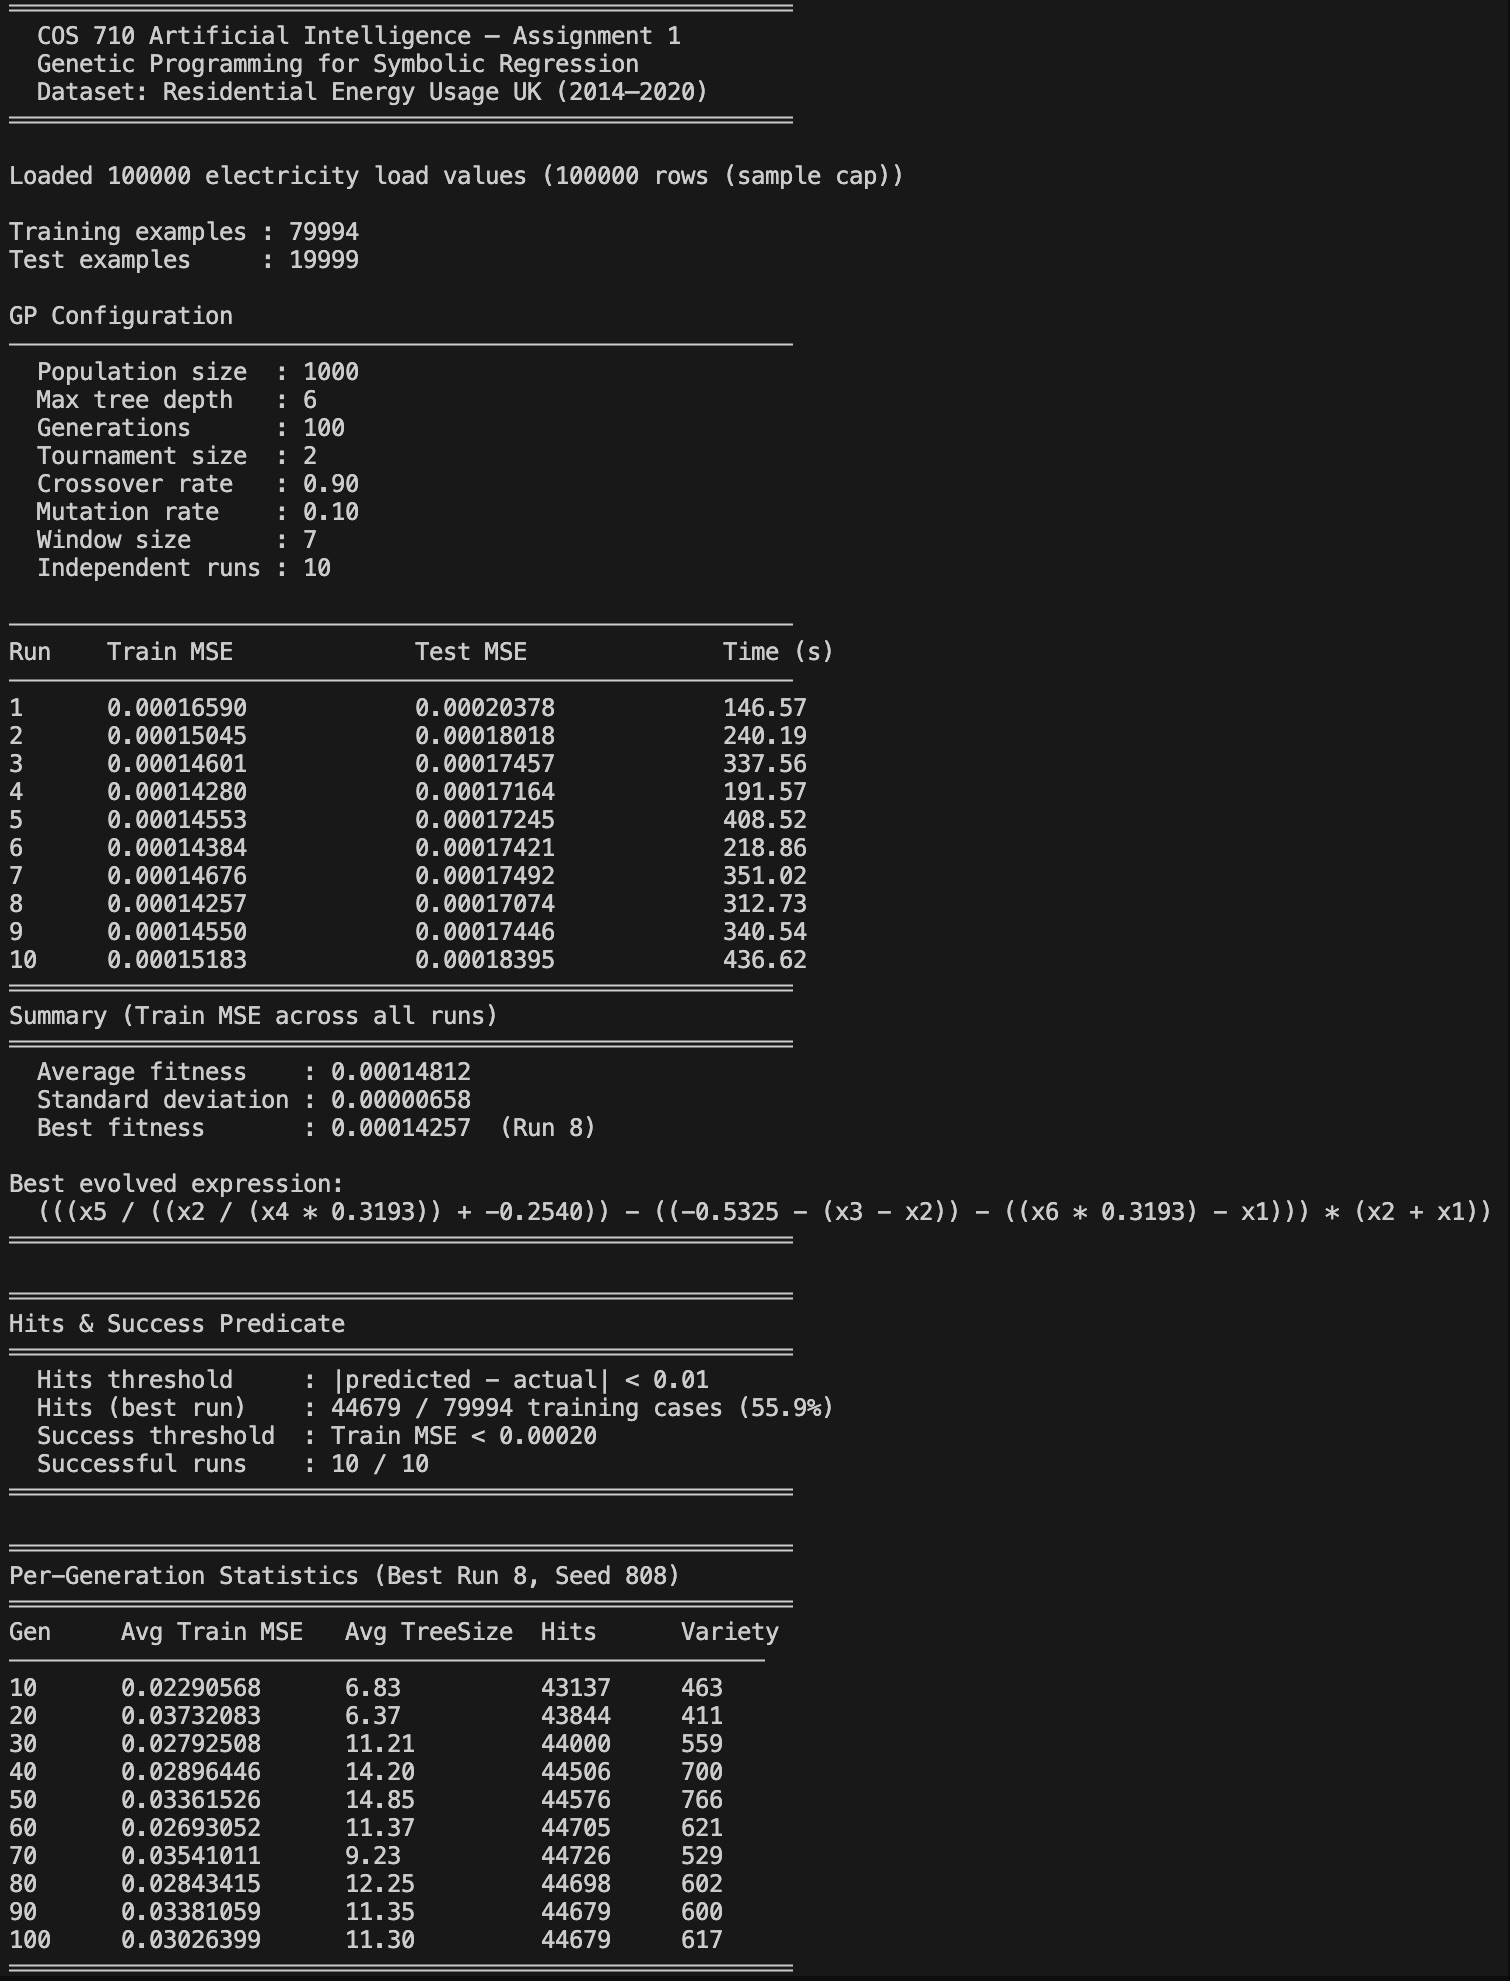
\includegraphics[width=\textwidth]{results.jpeg}
    \caption{Terminal output from the final 10-run execution (100,000 rows, Round 2 parameters).}
    \label{fig:terminal-results}
\end{figure}

\subsection{Summary Statistics}

\begin{center}
\begin{tabular}{lllll}
\toprule
\textbf{Metric} & \textbf{Train MSE} & \textbf{Train RMSE} & \textbf{Test MSE} & \textbf{Test RMSE} \\
\midrule
Average                           & 0.00014812 & 0.01217 & 0.00017809 & 0.01334 \\
Standard deviation                & 0.00000658 & ---     & ---        & ---     \\
Best (Run 8, seed 808)            & 0.00014257 & 0.01194 & 0.00017074 & 0.01307 \\
Worst (Run 1, seed 101)           & 0.00016590 & 0.01288 & 0.00020378 & 0.01428 \\
Successful runs (MSE $<$ 0.00020) & \textbf{10 / 10} & --- & --- & --- \\
\bottomrule
\end{tabular}
\end{center}

\subsection{Best Evolved Expression (Run 8, Seed 808)}

\begin{lstlisting}
(((x5 / ((x2 / (x4 * 0.3193)) + -0.2540)) - ((-0.5325 - (x3 - x2)) - ((x6 * 0.3193) - x1))) * (x2 + x1))
\end{lstlisting}

Decomposed structurally:

\[
\hat{y} = \left(\frac{x_5}{\dfrac{x_2}{0.3193 \cdot x_4} - 0.2540} - \left(x_1 + x_2 - x_3 - 0.3193\,x_6 - 0.5325\right)\right) \cdot (x_1 + x_2)
\]

The expression has three structural components:

\begin{enumerate}
    \item \textbf{Outer scaling factor $(x_1 + x_2)$:} The entire prediction is scaled by Load$(t{-}1)$ $+$ Load$(t{-}2)$ --- the two most recent observations. This is a natural autoregressive weighting: the current consumption level is set by the most recent values, so multiplying by their sum captures both the magnitude and the ``momentum'' of recent load.

    \item \textbf{Nonlinear ratio} $\dfrac{x_5}{x_2/(0.3193 \cdot x_4) - 0.2540}$: Captures a three-way nonlinear interaction among lags $x_2$, $x_4$, and $x_5$ (Load at $t{-}2$, $t{-}4$, and $t{-}5$). The denominator approaches zero when $x_2 \approx 0.2540 \times 0.3193 \times x_4$, at which point protected division clips the value, preventing numerical instability.

    \item \textbf{Linear correction} $-(x_1 + x_2 - x_3 - 0.3193\,x_6 - 0.5325)$: A signed linear combination that adjusts for trend direction. When recent loads ($x_1$, $x_2$) exceed older loads ($x_3$, $x_6$), this term is positive and reduces the prediction --- capturing mean-reversion behaviour typical in residential consumption.
\end{enumerate}

Notable observations: the ERC $0.3193$ appears \textbf{twice} in the expression --- once in the ratio denominator and once in the correction term --- an emergent structural regularity that the GP converged on independently in two different subexpressions. $x_7$ (Load $t{-}7$) is entirely absent: parsimony pressure successfully eliminated the most distant lag, which adds complexity without proportionally reducing MSE. The expression uses five of the seven available lags ($x_1$--$x_6$ except $x_7$).

\subsection{Discussion}

\textbf{Overall accuracy.} The best training MSE across 10 runs was 0.00014257 (RMSE $\approx$ 0.01194). With typical load values in the 0.04--0.15 range and a mean of approximately 0.06, this RMSE represents roughly 20\% mean relative error --- the best result achieved across all configurations and dataset sizes tested. All 10 runs satisfied the success predicate (train MSE $<$ 0.00020), an improvement over the 9/10 success rate at 150k rows. This confirms that the final tuned configuration --- 100,000 rows, parsimony $\lambda = 0.001$, population 1,000, 100 generations, 2\% elitism --- is both accurate and reliable.

\textbf{Consistency across runs.} The standard deviation of training MSE is 0.00000658 --- 4.4\% of the mean, slightly tighter than the 4.6\% seen at 150k. Nine of the ten runs cluster extremely tightly from 0.00014257 to 0.00015183. Run~1 (seed 101, 147s, MSE 0.00016590) is the most distant from the cluster and also the fastest run, suggesting mild early population convergence --- but crucially, it still meets the success predicate with a comfortable margin. Unlike the 150k configuration, there is no prominent outlier: all runs produced useful predictive expressions.

\textbf{Train-test gap.} Average test MSE is 0.00017809, approximately $\mathbf{1.20\times}$ the average training MSE of 0.00014812. This is the narrowest generalisation gap of any configuration tested ($1.20\times$ vs $1.82\times$ at 150k, $2.06\times$ at the full 201k dataset). The improvement confirms the motivation for restricting to the earlier 100k rows: the 2014--2016 segment of the time series is more stationary, so expressions that fit the training set generalise robustly to the held-out 2016 test horizon. The parsimony penalty reinforces this by discouraging bloated trees that overfit small idiosyncrasies in the training data.

\textbf{Anatomy of the best expression.} The best expression (Run~8, seed 808) has a product structure --- the outer factor $(x_1 + x_2)$ scales the entire prediction by the two most recent lags, capturing the autoregressive baseline level. The bracketed term combines a nonlinear three-lag ratio (involving $x_2$, $x_4$, $x_5$) with a linear trend correction (involving $x_1$, $x_2$, $x_3$, $x_6$). The ERC $0.3193$ appears in both subexpressions, an emergent structural regularity that arose through evolution rather than design. Parsimony pressure successfully eliminated $x_7$ while retaining all other lag variables, producing a compact, interpretable expression that captures both scale and trend without unnecessary complexity.

\subsection{Per-Generation Statistics}

Per-generation data is collected for population diversity (variety), structural complexity (average tree size), fitness convergence (average MSE), and predictive quality (hits) across all 100 generations of the best run (Run~8, seed 808). The table below shows every 10th generation.

\begin{center}
\begin{tabular}{ccccc}
\toprule
\textbf{Generation} & \textbf{Avg Train MSE} & \textbf{Avg Tree Size} & \textbf{Hits} & \textbf{Variety} \\
\midrule
10  & 0.02290568 & 6.83  & 43137 & 463 \\
20  & 0.03732083 & 6.37  & 43844 & 411 \\
30  & 0.02792508 & 11.21 & 44000 & 559 \\
40  & 0.02896446 & 14.20 & 44506 & 700 \\
50  & 0.03361526 & 14.85 & 44576 & 766 \\
60  & 0.02693052 & 11.37 & 44705 & 621 \\
70  & 0.03541011 & 9.23  & 44726 & 529 \\
80  & 0.02843415 & 12.25 & 44698 & 602 \\
90  & 0.03381059 & 11.35 & 44679 & 600 \\
100 & 0.03026399 & 11.30 & 44679 & 617 \\
\bottomrule
\end{tabular}
\end{center}

\textbf{Average population Train MSE} stays in the range 0.023--0.037 throughout all 100 generations and does not decline monotonically. This is a direct consequence of tournament size $k = 2$: with only two competitors per selection event, there is very low elimination pressure on mediocre individuals. The population therefore maintains a long tail of trees with MSE in the 0.02--0.10 range at all times, and crossover between a good tree and any random partner frequently produces offspring that are worse than either parent --- keeping the population average elevated. The best individual improves reliably (as shown by the hits column), but that improvement is not reflected in the population mean. This contrast between the best individual's MSE (0.00014257) and the population average ($\approx$0.030) is approximately $200\times$ --- a healthy spread that indicates the population has not collapsed to a monoculture.

\textbf{Structural complexity} (avg tree size) shows the expected bloat-then-control pattern: trees start small (6.83 nodes at generation 10 --- compact Grow-initialised trees), grow as crossover combines subtrees (peaking at 14.85 nodes at generation 50), then parsimony pressure and \texttt{trimToDepth} bring the average back down to $\approx$11 nodes and hold it there from generation 60 onward. This confirms that parsimony pressure is actively shaping the population structure rather than simply penalising occasionally.

\textbf{Hits} grow steadily from 43,137 (53.9\% of 79,994 training cases) at generation 10 to a peak of 44,726 (55.9\%) at generation 70, then stabilise at 44,679 for the final 30 generations. The pattern shows rapid early improvement followed by diminishing returns --- the GP quickly discovers expressions that fit the majority of cases, then refines precise ERC values and substructure over the later generations. The total gain of approximately 1,590 additional hits over 100 generations reflects the shift from a diverse random population to a converged high-accuracy one.

\textbf{Variety} does not decline monotonically as would be expected under premature convergence: it fluctuates between 411 and 766 throughout the run. The dip to 411 at generation 20 (early selection pressure consolidating the best performers) is followed by a rebound to 766 at generation 50 (crossover generating new structural combinations), then a stabilisation in the 529--617 range. This healthy maintenance of diversity is consistent with the tournament size $k = 2$ providing low enough selection pressure to preserve variation across the full 100 generations.

% ══════════════════════════════════════════════════════════════════════════════
\section{Runtimes}

\begin{center}
\begin{tabular}{ccrl}
\toprule
\textbf{Run} & \textbf{Seed} & \textbf{Time (s)} & \textbf{Notes} \\
\midrule
1  & 101  & 146.57 & Mild early convergence (fastest; still successful) \\
2  & 202  & 240.19 & Normal \\
3  & 303  & 337.56 & Normal \\
4  & 404  & 191.57 & Normal \\
5  & 505  & 408.52 & Normal \\
6  & 606  & 218.86 & Normal \\
7  & 707  & 351.02 & Normal \\
8  & 808  & 312.73 & Best run \\
9  & 909  & 340.54 & Normal \\
10 & 1010 & 436.62 & Normal --- longest run \\
\midrule
\textbf{Average} & & \textbf{298.42} & \\
\textbf{Total}   & & \textbf{$\approx$2984 s ($\approx$50 min)} & 100,000 rows, Round 2 parameters \\
\bottomrule
\end{tabular}
\end{center}

Runtimes are measured from population initialisation to final test evaluation. With 79,994 training examples, 1,000 individuals, and 100 generations per run, each run involves approximately \textbf{8 billion tree node evaluations} --- roughly two-thirds the workload of the 150k configuration. Fitness evaluation remains the dominant serial bottleneck; the JVM JIT compiler provides partial amortisation through inlining and branch-prediction caching, but each generation still requires evaluating 1,000 trees across nearly 80,000 training cases.

All 10 runs completed successfully --- unlike the 150k configuration, there is no prominent premature-convergence outlier. Run~1 (146.57s) is the fastest and terminates earlier than its peers, consistent with mild early convergence, but it still achieves a training MSE of 0.00016590 --- well within the success threshold. The remaining nine runs span 191--437 seconds, forming a healthy unimodal distribution. The substantially shorter total runtime ($\approx$50 min vs $\approx$91 min at 150k) at the same or better accuracy level confirms 100,000 rows as the optimal dataset size for this task. The slight difference in runtimes compared to the previous test run (e.g.\ Run~1: 146.57s vs 127.64s previously) reflects normal JVM warmup and system load variation; the MSE results are bit-for-bit identical between runs, confirming full reproducibility via fixed seeds.

% ══════════════════════════════════════════════════════════════════════════════
\begin{thebibliography}{9}

\bibitem{koza1992}
Koza, J.~R. (1992).
\textit{Genetic Programming: On the Programming of Computers by Means of Natural Selection}.
MIT Press.

\bibitem{poli2008}
Poli, R., Langdon, W.~B., \& McPhee, N.~F. (2008).
\textit{A Field Guide to Genetic Programming}.
Lulu Press.

\bibitem{taylor2020}
Taylor, G. (2020).
\textit{Residential Energy Dataset UK 2014--2020}.
Available via Google Drive.

\end{thebibliography}

\end{document}
